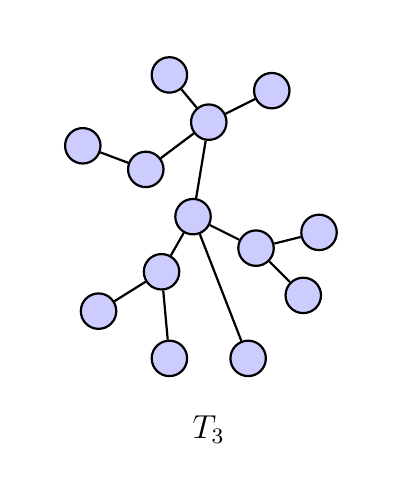
\begin{tikzpicture}[
  baseline=0pt,
  scale=1,
  vnode/.style={circle, draw=black, fill=blue!20, thick, inner sep=0pt, minimum size=4.5mm},
  edge/.style={thick, draw=black}
]
  \useasboundingbox (-2.3,-3.1) rectangle (2.3,2.4);

  % Posicionamiento de los 13 vértices
  \node[vnode] (u1) at (-0.5, 1.8) {};   % Vértice superior
  \node[vnode] (u2) at (0.0, 1.2) {};
  \node[vnode] (u3) at (0.8, 1.6) {};
  \node[vnode] (u4) at (-0.8, 0.6) {};
  \node[vnode] (u5) at (-1.6, 0.9) {};
  \node[vnode] (u6) at (-0.2, 0.0) {};
  \node[vnode] (u7) at (0.6, -0.4) {};
  \node[vnode] (u8) at (1.4, -0.2) {};
  \node[vnode] (u9) at (1.2, -1.0) {};
  \node[vnode] (u10) at (-0.6, -0.7) {};
  \node[vnode] (u11) at (-1.4, -1.2) {};
  \node[vnode] (u12) at (-0.5, -1.8) {}; % Vértice inferior 1
  \node[vnode] (u13) at (0.5, -1.8) {};  % Vértice inferior 2

  % Aristas (12 conexiones)
  \draw[edge] (u2) -- (u1);
  \draw[edge] (u2) -- (u3);
  \draw[edge] (u2) -- (u4); \draw[edge] (u4) -- (u5);
  \draw[edge] (u2) -- (u6);
  \draw[edge] (u6) -- (u7); \draw[edge] (u7) -- (u8); \draw[edge] (u7) -- (u9);
  \draw[edge] (u6) -- (u10); \draw[edge] (u10) -- (u11); \draw[edge] (u10) -- (u12);
  \draw[edge] (u6) -- (u13);

  % Etiqueta
  \node[font=\large] at (0,-2.7) {$T_3$};
\end{tikzpicture}
